%% LyX 2.4.2.1 created this file.  For more info, see https://www.lyx.org/.
%% Do not edit unless you really know what you are doing.
\documentclass[12pt,english]{beamer}
\usepackage{mathpazo}
\renewcommand{\familydefault}{\rmdefault}
\usepackage[T1]{fontenc}
\usepackage[latin9]{inputenc}
\setcounter{secnumdepth}{3}
\setcounter{tocdepth}{3}
\usepackage[active]{srcltx}
\usepackage{amsthm}
\usepackage{amsmath} 
\usepackage{amssymb}
\usepackage[authoryear]{natbib}
\usepackage{graphicx}

\makeatletter
%%%%%%%%%%%%%%%%%%%%%%%%%%%%%% Textclass specific LaTeX commands.
% this default might be overridden by plain title style
\newcommand\makebeamertitle{\frame{\maketitle}}%
% (ERT) argument for the TOC
\AtBeginDocument{%
  \let\origtableofcontents=\tableofcontents
  \def\tableofcontents{\@ifnextchar[{\origtableofcontents}{\gobbletableofcontents}}
  \def\gobbletableofcontents#1{\origtableofcontents}
}
\theoremstyle{definition}
\newtheorem*{example*}{\protect\examplename}
\theoremstyle{definition}
\newtheorem*{defn*}{\protect\definitionname}
\theoremstyle{plain}
\newtheorem*{thm*}{\protect\theoremname}

%%%%%%%%%%%%%%%%%%%%%%%%%%%%%% User specified LaTeX commands.
\AtBeginDocument{%
   \let\origtableofcontents=\tableofcontents
   \def\tableofcontents{\@ifnextchar[{\origtableofcontents}{\gobbletableofcontents}}
   \def\gobbletableofcontents#1{\origtableofcontents}
 }\usepackage[english]{babel}
\usepackage{babel}

%\usetheme{Boadilla}
\usetheme{Madrid}
\setbeamertemplate{navigation symbols}{}
% \usecolortheme{orchid}
\usecolortheme{spruce}
% \usecolortheme{beaver}

\setbeamercovered{transparent}

\usepackage{colortbl}

\usefonttheme[onlymath]{serif}
%%%%%%%%%%%%%%%%%%%%%%%%

% For tables
\usepackage{multirow}
\usepackage{array}
\usepackage{rotating}
\usepackage{longtable}
\usepackage{float}
\usepackage{booktabs}


% For figures
\usepackage{caption}
\usepackage{subcaption}

\makeatother

\usepackage{babel}
\providecommand{\definitionname}{Definition}
\providecommand{\examplename}{Example}
\providecommand{\theoremname}{Theorem}

% 定义命令 \RomanNum 和 \romanNum
\newcommand{\RomanNum}[1]{\uppercase\expandafter{\romannumeral #1\relax}} % 大写罗马数字
\newcommand{\romanNum}[1]{\romannumeral #1\relax} % 小写罗马数字

\begin{document}
\title[Limited]{Models of Limited Dependent Variables}
\author[]{Zhentao Shi}
\date[]{The Chinese University of Hong Kong}

\makebeamertitle



\begin{frame}{Fundamental Task}

        \begin{itemize}
            \item Use $X$ to predict $y$
        \item Beyond continuous random variables
        \begin{itemize}
            \item Binary
            \item Multi-responses 
            \item Integer
            \item Mixed type: censoring, truncation
            \item Self-selection
        \end{itemize}

\bigskip
            
        \item Applied microeconomics
        \item Biostatistics
            
        \end{itemize}
\end{frame}

\begin{frame}[plain]{Unification}
    \begin{center}
        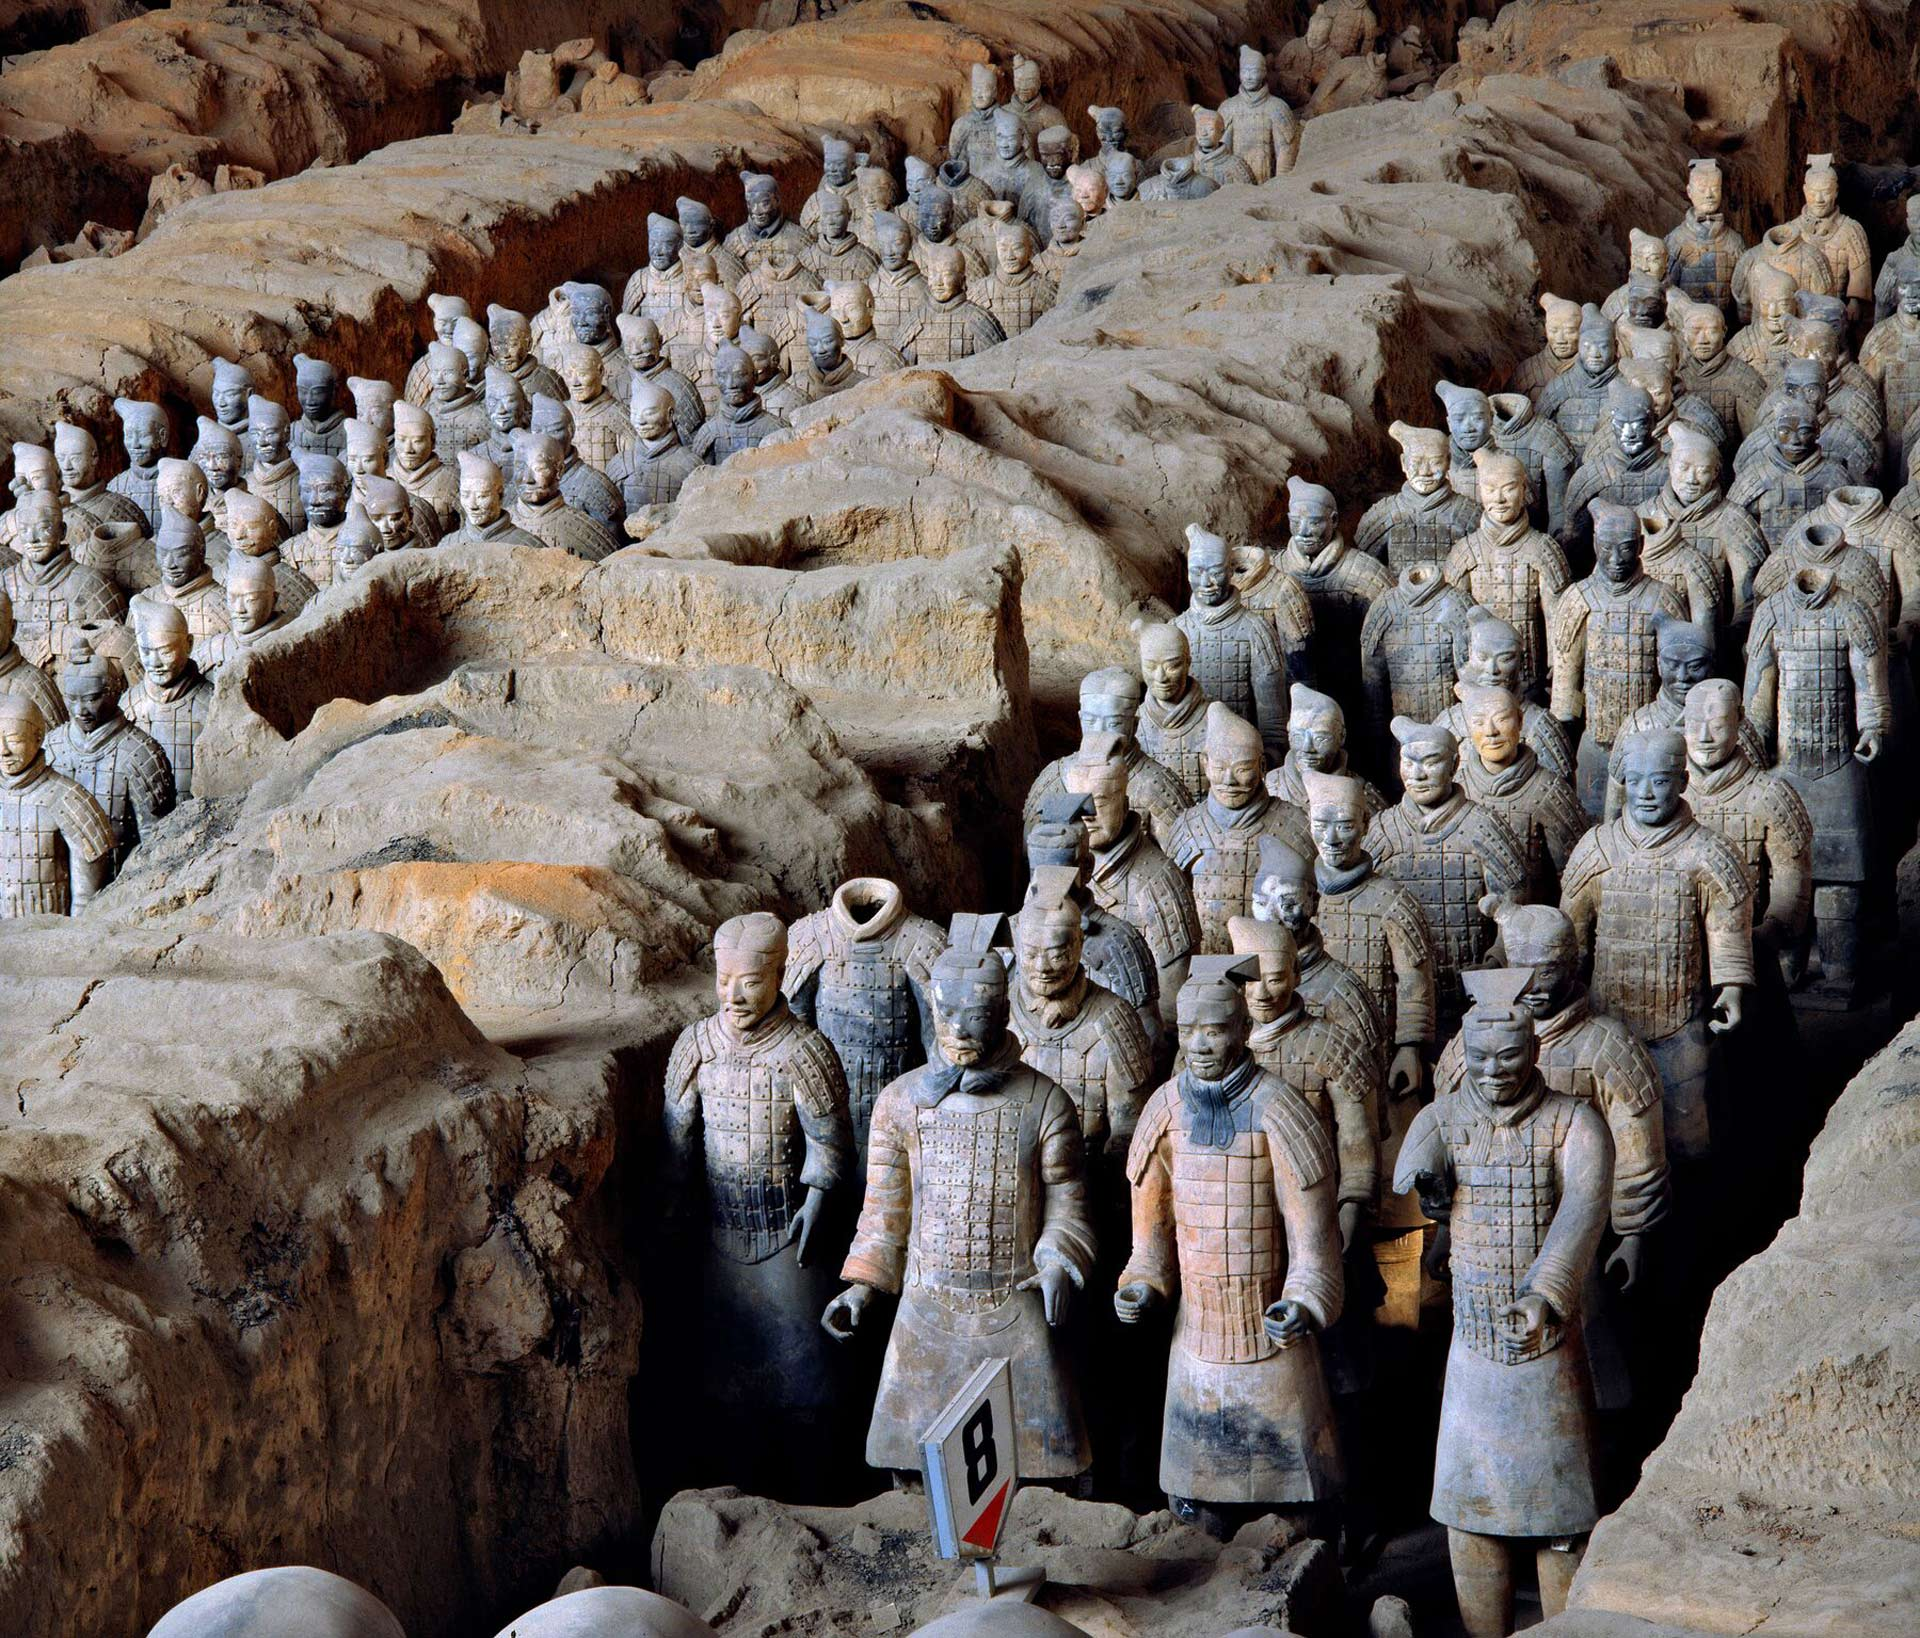
\includegraphics[width = \textwidth]{fig/terracotta_warriors.jpg}
    \end{center}
\end{frame}



\begin{frame}{Panoramic View}
    \begin{itemize}
        \item MLE is the unifying framework
        \item Regressors $X_i$ enter the model in a single index $X_i'\beta$
        \item Functional forms are convenient choices
        \item Economic interpretation as utilities
    \end{itemize}
\end{frame}


\section{Binary Choices}
\frame{\sectionpage}




\begin{frame}{Binary Outcome}
    \begin{minipage}{0.6\textwidth} % Left side for text
        \begin{itemize}
            \item Outcome $y_{i} \in \{ 0, 1\}$
            \item Classification
                \begin{itemize}
                    \item Unsupervised learning: k-means algorithms
                \end{itemize}
            \item Binary regression (Supervised learning)
            \begin{itemize}
                \item College entrance
                \item Marriage
                \item Loan decision
                \item Spam filter
            \end{itemize}
        \end{itemize}
    \end{minipage}%
    \hfill
    \begin{minipage}{0.4\textwidth} % Right side for image
        \centering
        
\includegraphics[width=0.8\textwidth]{fig/yin_yang.png}
    \end{minipage}
\end{frame}






\begin{frame}{Linear Probability Models}

\begin{itemize}
    \item Keep using linear regression $y_i = X_i^{'} \beta + \varepsilon_i$
    \item Conditional mean $$\Pr \left[y_{i} = 1 \mid X_{i}\right] = E\left[y_{i} = 1 \mid X_{i}\right] = X_{i}^{'} \beta$$
    \item Error term $\varepsilon _{i} \in \{  - X_{i}^{'} \beta, \, 
    1- X_{i}^{'} \beta \} $ is binary.
    \item Conditional heteroskedastic.
    \item Predicted range: $E\left [y_{i} = 1 \mid X_{i} \right] = X_{i}' \beta$ can go beyond $\left[0,1\right]$.
    \begin{itemize}
        \item $X_{i}^{'} \beta$ is a ``single index''.
    \end{itemize}
\end{itemize}
\end{frame}



\begin{frame}{Generalized Linear Model}
    \begin{itemize}
        \item To ensure predicted probability inside \( [0,1] \), pick some \( G(\cdot ) : \mathbb{R} \to \left[ 0, 1\right] \) to model 
        \[
        E\left( y _{i} = 1 \mid X_{i} \right) = G (X_i^{'} \beta) 
        \]
        \item Popular choices
        \begin{itemize}
           \item Probit: \( G(x) \sim \text{Normal cdf} \)
           \item Logit: \( G\left(x\right) \sim \text{Logistic cdf} \)
        \end{itemize}
        \item Facts about Logistic CDF
        \begin{itemize}
            \item \( \Lambda = \Lambda \left(x\right) = \frac{1}{1 + \exp \left(-x\right)} \)
            \item \( \frac{\mathrm{d} \Lambda }{\mathrm{d} x} = \Lambda \left(1-\Lambda \right) \)
        \end{itemize}
    \end{itemize}
    \begin{picture}(0,0)
        % Adjust the position and scale of the image as needed
        \put(185,-5){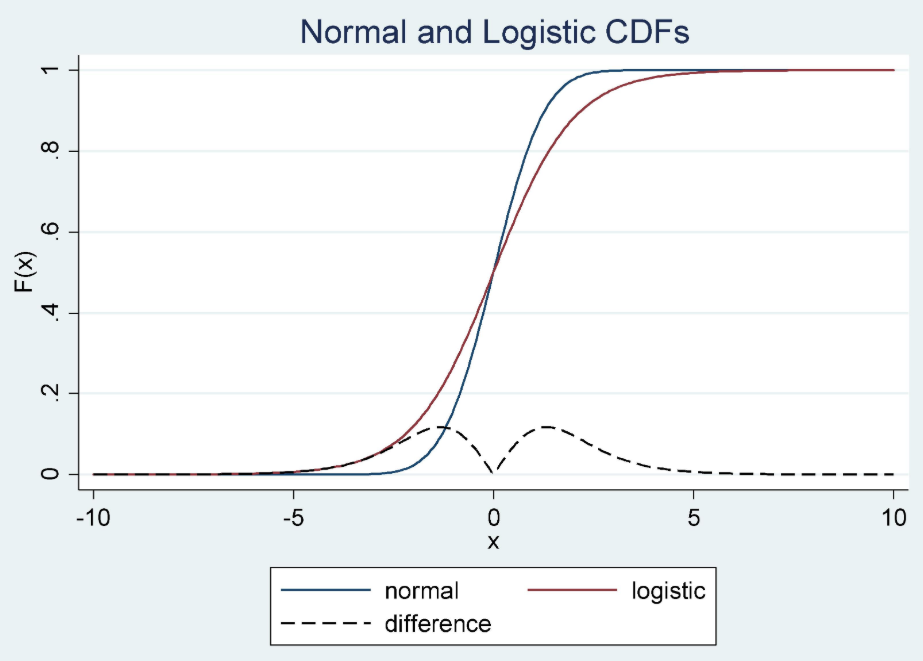
\includegraphics[width=0.45\textwidth]{fig/logistic_normal.png}}
    \end{picture}  
\end{frame}
\begin{frame}{Latent Utility Model}

\begin{itemize}
    \item Latent utility $y^{*} = X_{i}^{'} \beta + \varepsilon _{i}$
    \item Observed outcome $y = \mathbb{I}\left\{ y_{i} ^{*} \ge 0 \right\}$
    \item If $\varepsilon _{i} \mid X_i \sim \text{Logistic}$, then
    \begin{align*}
        \Pr\left(y_i = 1 \mid X_i \right) &= \Pr \left(X_i^{'} \beta + \varepsilon _{i} \ge 0 \mid X_i\right)\\
        & = \Pr \left( - \varepsilon _{i} \le X_{i}^{'} \beta \mid X_{i}\right)\\
        & = \Lambda \left(X_i^{'} \beta\right)
    \end{align*}
    \item The scale of $\beta$ is not identifiable
\end{itemize}


\end{frame}
\begin{frame}{Log-Likelihood}

A sample of $N$ observations of $(y_i, X_i)$
    \begin{align*}
        L(\beta) &= \prod_{y_i = 1 } \Lambda \left( X_i ^{'} \beta \right)\cdot \prod_{y_i = 0} \left(1 - \Lambda \left(X_{i}^{'} \beta \right)\right)\\
        &= \prod_{i =1}^{N}\left\{ \Lambda \left(X_i^{'} \beta \right) \right\} ^{y_i} \left\{ 1- \Lambda \left( X_{i}^{'} \beta \right) \right\} ^{1-y_{i}}
    \end{align*}

Log-likelihood
    \[\ell_n \left( \beta \right) = \sum_{i =1}^{N} \left\{ y_i \log \left( \Lambda \left( X_{i}^{'}\beta \right) \right) + \left( 1 - y_{i} \right)  \log \left( 1 - \Lambda \left( X_i' \beta \right) \right)\right\}\]
    
    
\end{frame}

\begin{frame}{Properties}


    \begin{itemize}
    \item The score
    \begin{align*}
        S_N(\beta) &= \sum_{i = 1}^{N}\left\{ \frac{y_i}{\Lambda_i}\cdot \Lambda_{i}\left( 1 - \Lambda _i \right) X_{i} - \frac{\left( 1- y_{i} \right)}{1 - \Lambda_{i}} \cdot \Lambda_{i} \left( 1-\Lambda_{i} \right) X_{i}\right\}\\
        &= \sum_{i=1}^{N}\left\{ y_{i} \left( 1- \Lambda_{i} \right) - \left( 1-y_{i} \right) \Lambda_{i}\right\} X_{i}\\
        &= \sum_{i =1}^{N}\left( y_{i} - \Lambda _{i} \right)X_{i} 
    \end{align*}
    \item Negative-definite second derivative
    \[\frac{\partial L \left( \beta \right)}{\partial \beta \partial \beta ^{'}} = - \sum_{i=1}^{N} \Lambda_{i}\left( 1 - \Lambda_{i} \right) X_{i} X_{i}'.\]

        \item Globally concavity implies uniqueness of maximizer.
    \end{itemize}
\end{frame}


\begin{frame}{Goodness of Fit for Binary Classification}
     $$\text{McFadden} R^{2} = 1- \log L_{1} / \log L_{0}$$
    \begin{itemize}
        \item $\log L_{1}$: maximum of likelihood
        \item $\log L_{0}$: the null model (no $X$, intercept only)
            \[\log L_{0} = N_1 \log \hat{p}_1 + \left( N-N_{1} \right)\log \left( 1- \hat{p}_1 \right) \]
            where $\hat{p}_1 = N_{1} / N$
        \item $\log L_{0} < \log L_{1} < 0 \Rightarrow \frac{\log L_{1}}{\log L_{0}} \in \left[0,1  \right]$                
    \end{itemize}
\end{frame}

\begin{frame}{Maximum Likelihood}
\begin{itemize}
    \item All familiar properties of ML hold
    \item Misspecification?
    \item Choices of loss functions
\end{itemize}
    
\end{frame}


\begin{frame}{Prediction and Evaluation}
   Natural prediction: \[\hat{y_{i}} = 1 \,\text{if}\, \Pr\left( y_{i} \mid X_{i} \right) \ge 0.5\]

   Outcomes: $n_{11}$: correct positive; $n_{01}$: false positive
    \begin{table}
        \centering
        \begin{tabular}{rr|ccc}
            & & $\hat{y}_i = 0$ & $1$ & Total \\
            \hline
              & $y_{i}=0$ & $n_{00}$ & $n_{01}$ & $N_{0}$ \\
            & $1$ & $n_{10}$ & $n_{11}$ & $N_{1}$ \\
            \hline
            & Total &&& $N$ 
        \end{tabular}
    \end{table}
    \begin{itemize}
        \item Hendrick-Merton: $\frac{n_{00}}{N_{0}} + \frac{n_{11}}{N_{1}}$
        \item Kuiper Score: $\frac{n_{11}}{N_{1}} - \frac{n_{01}}{N_{0}}$
    \end{itemize}
\end{frame}




\section{Multiple Choices}
\frame{\sectionpage}


\begin{frame}{Ordered Response}
    \begin{itemize}
        \item More than two categories
        \item Categories are naturally ordered

\textcolor{red}{add the picture "caste.webp" into this slide. I attempted to change it to "png" and use the following code, but it didn't work.}

%\begin{center}
%    
\includegraphics[width=0.7\textwidth]{fig/caste.png}
%\end{center}

    \end{itemize}
\end{frame}


\begin{frame}{Utility}
    \begin{itemize}

        \item Latent utility: $$y_{i}^{*} = X_{i}' \beta + \varepsilon_{i}$$ while the observed outcome  $$y_{i} = j, \, \text{if}\, r_{j} < y_{i}^{*} \le r_{j+1}$$

    \begin{itemize}
        \item Normalization is needed for identification
        \item $M$ categories
        \item $\gamma_{1} = - \infty,\, \gamma_{M+1} = + \infty, \, \gamma_{2} = 0$
    \end{itemize}
        
    \end{itemize}
\end{frame}



\begin{frame}{Probability}
    \begin{itemize}

        \item Unknown parameters: $\left( \beta, \gamma_{3}, \dots, \gamma_{M} \right)$
    \end{itemize}
    \begin{align*}
        P_{ij} & = \Pr\left( \gamma_{j} < y_{i}^{*} \le \gamma_{j+1} \mid X_{i}\right)\\
        & = \Pr \left( y_{i}^{*} \le \gamma_{j+1} \mid X_{i} \right) - \Pr \left( \gamma_{j} \le y_{i}^{*} \mid X_{i} \right)\\
        & = \Pr \left( \varepsilon_{i} \le \gamma_{j+1} - X_{i}^{'} \beta \right) - \Pr \left( - \varepsilon_{i} \le X_{i}^{'} \beta - \gamma_{j} \mid X_{i} \right)
    \end{align*}
\end{frame}

\begin{frame}{Likelihood}
    \begin{itemize}
        \item Unobservable error $\varepsilon_{i} \mid X_{i}$ is assumed to be either logistic or normal
        \item Likelihood of individual observation \[ \Pr \left( y_i = j \right) = \sum_{j=1}^{M} P_{ij} \mathbb{I}\left\{ y_j = j \right\}\]
        \item Likelihood of the $N$-observation sample 
    \[ L\left( \theta \right) = \prod_{i =1} ^{N} \Pr \left( y_j = j \right)\]
    \end{itemize}
    
\end{frame}



\begin{frame}{Multinomial Choice}
  

\begin{center}
    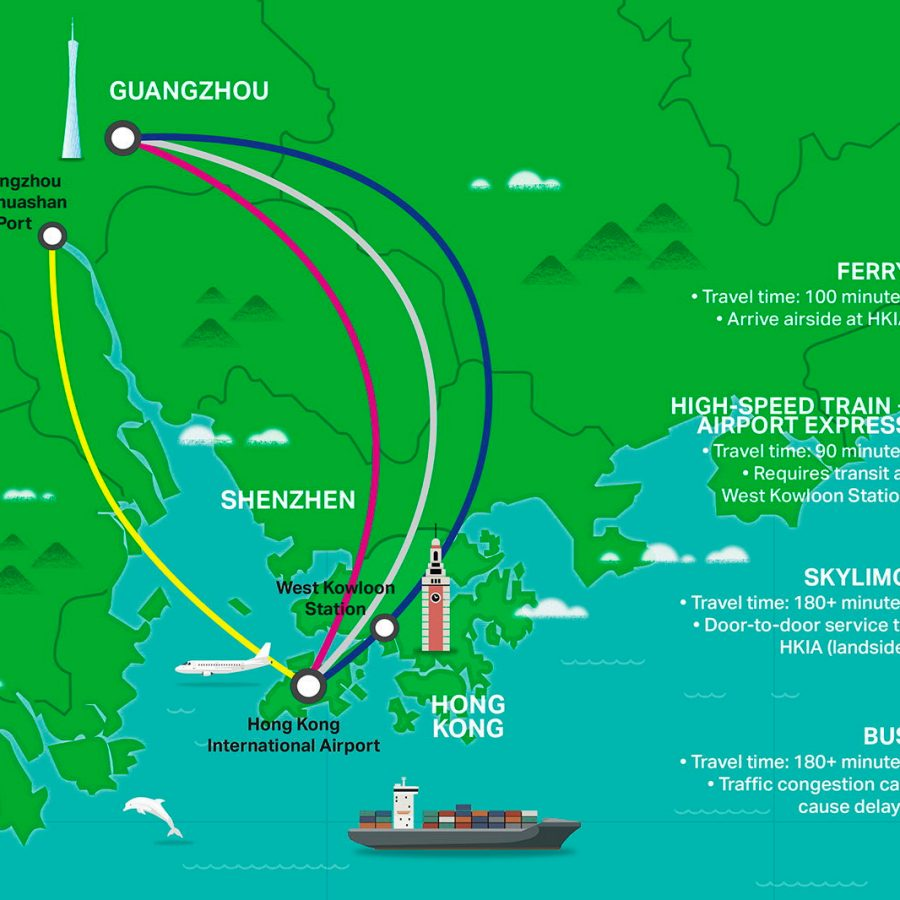
\includegraphics[width=0.65\textwidth]{fig/Guangzhou.jpg}
\end{center}
    
\end{frame}



\begin{frame}{Multinomial Choice}
    \begin{itemize}
        \item How do you travel from Hong Kong to Guangzhou? By bus, train, or plane?
        \item Machine learning: handwritten numbers
        \item Level Individual-choice utility
        $$\mu_{ij} = W_{ij}^{'} \beta + Z_{i}^{'} \beta_{j}$$
        \item Choice-specific regressors $W_{ij}$
        \begin{itemize}
            \item e.g.~Distance to stations ($\beta$ is value of time)
        \end{itemize}
        \item Choice-invariant regressors $Z_{i}$
        \begin{itemize}
            \item e.g.~Motion sickness ($\beta_j$ is the effect; bus is bad)
        \end{itemize}
        
    \end{itemize}    
\end{frame}

\begin{frame}{Latent Utility}
    \begin{itemize}
        \item $y_{ij}^{*} = \mu_{ij} + \varepsilon _{ij}$, for $\left(\varepsilon_{ij}\right)_{j=1}^{M}$
        \item $y_{j} = \mathbb{I}\left\{ j: y_{ij}^{*} \ge y_{ik},\,\text{for }\, k = 1, \dots, M \right\}$
        \item $\Pr \left( y_{j} = j \mid \mu_{i1}, \dots, \mu_{iM} \right) = \Pr \left( y_{ij}^{*} \ge y_{i1}^{*}, \dots, y_{ij}^{*} \ge y_{iM}^{*} \right)$
        \item The probability depends on the joint distribution of $\left( \varepsilon_{ij} \right)_{j=1}^{M}$
        \item If $\varepsilon _{ij} \sim $ Type \RomanNum{1} extreme value distribution and $\varepsilon_{ij}$ i.i.d.~across choices, then
        \[\Pr\left( y_{ij} = j \mid \mu_{i1}, \dots, \mu_{iM} \right)= \frac{\exp\left( \mu_{ij}\right)}{\sum_{k=1}^{M}\exp \left( \mu_{ik}\right)}\]
    \end{itemize}
\end{frame}



\begin{frame}{Normalization}
    \begin{itemize}
        \item $\mu_{i1} = 0$ for all $i$
        \item Equivalent to $\beta_{j=1} = 0$ (including intercept)
        \item Parameters: $\left( \beta;   \beta_2, \beta_3, \dots, \beta_M\right)$
    \[L\left( \theta \right) = \prod_{i=1}^{n} \left\{ \sum_{j=1}^{M} \mathbb{I} \left( y_{ij} = j \right)\left( \frac{\exp \left( \mu_{ij} \right)}{1 +  \sum_{k=2}^{M} \exp \left( \mu_{ik} \right)} \right) \right\}\]
    
        \item Again, it is about a convenient choice of loss function
    \end{itemize}

\end{frame}

\begin{frame}{Independence of Irrelevant Alternative}
    \begin{itemize}
        \item The concise from leverages that $\varepsilon_{ij}$ is i.i.d. across choices
        \item Dilemma of ``red bus'' versus ``blue bus''
        \item Must pay attention to the specification of choice set
        \item There are methods to fix it; still depending on choices.
    \end{itemize}
\end{frame}


\section{Integer Outcomes}
\frame{\sectionpage}


\begin{frame}{Counting Model}
\begin{itemize}
    \item Outcomes take non-negative integers
    \begin{itemize}
        \item Number of children
        \item Number of hospital visits
        \item Number of patents
    \end{itemize}
    \item Poisson model: 
$y \sim \text{Poisson}(\lambda)$:
$$
\Pr(y = k) = \frac{\mathrm{e}^{-\lambda} \lambda^k}{k!}, \mathrm{ for }\, \, k=0,1,2,\ldots
$$
    \item Poisson regression: single index $\lambda_i = X_i'\beta$ gives log-likelihood
$$
\log \Pr(y_i | X_i) =  -\exp(X_i'\beta) + y_i\cdot X_i'\beta - \log k!
$$
\end{itemize}
\end{frame}



\begin{frame}{Poisson MLE}
\begin{itemize}
    \item Log-likelihood function of an $N$-observation sample:
    \[
    \ell_N(\beta) = \log \Pr( \mathbf{y} | \mathbf{X}; \beta ) = -\sum_{i=1}^n \exp(X_i'\beta) + \sum_{i=1}^n y_i X_i'\beta.
    \]
    
    \item Score:
    \[
    s_N(\beta) = \frac{\partial \ell(\beta)}{\partial \beta} = -\sum_{i=1}^n \exp(X_i'\beta)X_i + \sum_{i=1}^n y_i x_i.
    \]

    \item Second derivative is negative definite:
    \[
    \frac{\partial^2 \ell(\beta)}{\partial \beta \partial \beta'} = -\sum_{i=1}^n \exp(X_i'\beta) X_i X_i'
    \]

    \item \( \ell_N(\beta) \) is strictly concave in \( \beta \).

\end{itemize}
\end{frame}



\begin{frame}{Pseudo Poisson MLE}

\begin{itemize}
    \item Conditional mean model $E[y|X] = \exp (X'\beta)$
    \item If $y$ is continuously distributed, the Poisson model must be misspecified
    \item e.g., Bilateral international trade between pairs of countries.
\end{itemize}
\end{frame}


\section{Incomplete Data}
\frame{\sectionpage}



\begin{frame}{Censored Data}
    \begin{itemize}
        \item Latent utility: $y_{i}^{*} = X_{i}^{'} \beta + \varepsilon_{i}$
        \item Observed outcome: 
        $\left\{\begin{matrix}
          y_{i} = y_{i}^{*},& \text{if} \, y_{i} >c\\
          y_{i} = c,&\text{if} \, y_{i} \le c
        \end{matrix}\right.$
        \item Tobit I model

        \item e.g.~Minimal wage
            \begin{itemize}
                \item Pull up the wage
            \end{itemize}
    \end{itemize}
\end{frame}

\begin{frame}{Probabilities}
    \begin{itemize}
        \item Assume $\varepsilon _{i} \mid X_{i} \sim N\left( 0, \sigma ^{2} \right)$
        \item The probability mass \begin{align*}
            \Pr \left( y_{i} = c \right)& = \Pr \left( y_{i}^{*} \le c \right) = \Pr \left( X_{i}^{'} \beta + \varepsilon _{i} \le c \right)\\
            & = \Pr \left( \frac{\varepsilon_{i}}{\sigma} \le \frac{c-X_{i}^{'} \beta}{\sigma} \right)  = \Phi \left( \frac{c - X_{i}^{'} \beta}{\sigma}\right)
        \end{align*}
        where $\Phi(\cdot)$ is the CDF of $N(0,1)$.
        \item The density of the continuous region remains the same.
    \end{itemize}
\end{frame}


\begin{frame}{Likelihood}

The likelihood consists of two components:
    \begin{align*}
        f\left( y_{i} \mid X_{i} \right) &= \Phi \left( \frac{c- X_{i}^{'} \beta}{\sigma} \right) \times \mathbb{I} \left( y_{i} = c \right) \\
        &+ \frac{1}{\sqrt{2 \pi}\sigma} \exp \left( -\frac{1}{2\sigma^{2} } \left( y_{i} - X_{i}^{'} \beta \right)^{2}\right) \times \mathbb{I} \left(y_{i} > c \right)
    \end{align*}
    \begin{itemize}
        \item Mixed type of discrete and continuous random variable
        \item Mixed of probability mass function and density
        \[ \int_{-\infty}^{\infty} f\left( y \mid X \right)\mathrm{d} y =1\]
    \end{itemize}
\end{frame}


\begin{frame}{Truncation}
    \begin{itemize}
        \item If data of those with $y_i = c$ are completely unobservable
        \item We have data $\left( Y_{i}, X_{i} \right)$ for those $y_{i} > c$ only.
        \item The likelihood with a condition on the outcome:
        \[f\left( y_{i} \mid y_{i} \ge c, X_{i} \right) = \frac{\frac{1}{\sqrt{2 \pi}\sigma} \exp \left( -\frac{1}{2\sigma^{2} } \left( y_{i} - X_{i}^{'} \beta \right)^{2}\right)}{1- \Phi \left( \frac{c-X_{i}^{'} \beta }{\sigma} \right)}\]
        \item Due to truncation, OLS cannot consistently estimate $\beta$
        \item Must use MLE
    \end{itemize}
\end{frame}


\begin{frame}{Tobit \RomanNum{2} Models}
    \begin{itemize}
        \item Wage (continuous): $y_{i}^{*} = x_{1i}^{'} \beta_{1} + \varepsilon  _{1i}$
        \item Choice (binary) : $h_{i}^{*} = x_{2i}^{'} \beta_{2} + \varepsilon _{2i}$ and the observed outcome 
        \[
         h_i = \left\{\begin{matrix}
          1,& \text{if } \, h_{i}^{*} \ge 0\\
          0,&\text{otherwise} 
        \end{matrix}\right.
        \]
        \item Observe $y_i = y_i^*$ if $h_i = 1$
        \item The two equations have different regressors, coefficients and and errors terms.
        \item More flexible than the Tobit I model
    \end{itemize}
\end{frame}

\begin{frame}{Conditional Expectation}
    \begin{itemize}
        \item Assume $\begin{pmatrix}
            \varepsilon_{1i}\\
            \varepsilon_{2i}
        \end{pmatrix} \sim N\left( \begin{pmatrix}
            0\\
            0
        \end{pmatrix}, \begin{pmatrix}
            \sigma_{11}^{2} & \sigma_{12} \\
            \sigma_{12} & 1
        \end{pmatrix} \right)$ \\
        where $\sigma_{22} = 1$ is a normalization
        \item Parameter $\theta = (\beta_1, \beta_2, \sigma_{11}^2, \sigma_{12})$, can be estimated by MLE \pause
        \item The conditional mean
        \begin{align*}
            E\left( y_{i}^{*} \mid h_{i} =1 \right) & = x_{1i}' \beta + E \left( \varepsilon_{1i} \mid h_{i} =1 \right) = x_{1i}' \beta + \sigma_{12} \lambda \left( x_{2i}' \beta_{2} \right)
        \end{align*}
        due to the joint normality, where $\lambda\left( x \right) = \phi \left( x \right) / \Phi \left( x \right)$ is called the \textbf{inverse Mill's ratio}. $\phi(\cdot)$ is the pdf of $N(0,1)$
        \item The regression model can be estimated by ``Heckit''.
    \end{itemize}
\end{frame}

\begin{frame}{Summary}
\begin{itemize}
    \item Binary choice
    \item Multiple choices: ordered or unordered
    \item Poission regression
    \item Censored data and truncated data
    \item Selection model

    \bigskip
    \item All are applications of MLE
\end{itemize}
    
\end{frame}


\end{document}